\section{2048}

2048 is played on a $4 \times 4$ grid.
The objective of the original 2048 game is to reach a 2048-tile by moving and merging
the tiles on the board according to the rules below.
In an initial state (Fig.~\ref{fig:game}), two tiles are placed randomly each with a number 2 (with probability $0.9$) or 4 (with probability $0.1$).
The player selects a direction (either up, right, down, or left), and then all the tiles will move in the selected direction.
When two tiles of the same number collide, they create a tile with the sum value and the player gets the sum as the score.
Here, the merges occur from the far side and newly created tiles do not merge again on the same move: move to the right from \verb*|222 |, \verb*| 422| and \verb*|2222| results in
\verb*|  24|, \verb*|  44|, and \verb*|  44|, respectively.
Note that the player cannot select a direction in which no tiles move nor merge.
After each move, a new tile appears randomly at an empty cell with a number 2 (with probability $0.9$) or 4 (with probability $0.1$).
If the player cannot move the tiles in any direction, the game ends.

Since a turn in 2048 consists of two steps, we introduce the two notions, namely \emph{state} and \emph{afterstate}~\cite{SzJa14}, which are shown in Fig.~\ref{fig:states-and-afterstates}.
\begin{itemize}
 \item A \emph{state} $s_t$ is a board (and score) at which the player selects a move.
 \item An \emph{afterstate} $s'_t$ is a board (and score) after the slide-and-merge step and before a new tile appears.
\end{itemize}

\begin{figure}[t]
  \begin{center}
    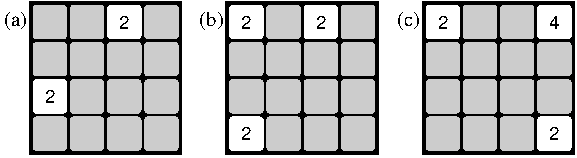
\includegraphics[width=.95\linewidth]{figures/2048RLJIP-1.pdf}\\[5pt]
  \begin{minipage}{.9\linewidth}
  \begin{enumerate}
   \item[(a)] An initial state. Two tiles are placed randomly.
   \item[(b)] After the first move: \emph{up}. A new 2-tile appears at the lower-left corner.
   \item[(c)] After the second move: \emph{right}. Two 2-tiles are merged to a 4-tile, and score 4 is given. A new tile appears at the upper-left corner.\\
  \end{enumerate}
  \end{minipage}
  \end{center}
 \caption{Process of game 2048~\cite{KoMa19}}
 \label{fig:game}
\end{figure}

\begin{table}[t]
 \caption{Score and number of moves when a tile is first created}
 \label{table:achievement}
 \centering\begin{tabular}{rrr}
\hline
\hline
  tile &     score  &   moves \\
\hline
  2048 &    20\,000 &     950 \\
  4096 &    44\,000 &  1\,900 \\
  8192 &    97\,000 &  3\,800 \\
 16384 &   210\,000 &  7\,500 \\
 32768 &   450\,000 & 15\,000 \\
\hline
 \end{tabular}
\end{table}

% 図\ref{afterstate2048}は,初期局面から始まるゲームの流れにおいて,state,afterstate,progress を図示したものである.
